Let's consider the following procedure: for some matrix $M$, find all eigenvalues $\lambda_j$, ordered in ascending order, and determine the $r$-parameter \cite{wei_characterization_2020}
\begin{equation}
    r \overset{\mathrm{def}}{=}  \left\langle \frac{\min(\delta_j, \delta_j+1)}{\max(\delta_j, \delta_{j+1})} \right\rangle_j,
    \hspace{10 mm} 
    \delta_j = \lambda_{j+1}-\lambda_j.
    \label{eq:rparam}
\end{equation}
We can immediately note several such properties that it is not sensitive to transformations of the form $M \to \alpha_1 M + \alpha_2 \1$, moreover, as we will notice later, it is not sensitive to many things.


\begin{figure}[h]
    \centering
    \addletter{107}{a}
    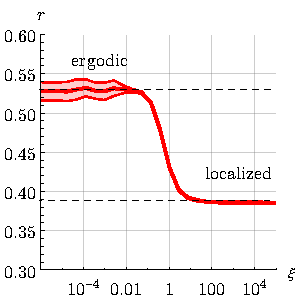
\includegraphics[width=0.225\textwidth]{imgs/erg_reg_add1.pdf}
    \hspace{10 mm} 
    \addletter{107}{b}
    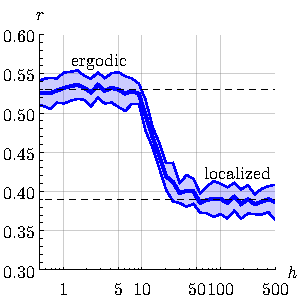
\includegraphics[width=0.225\textwidth]{imgs/erg_reg_add2.pdf}
    \caption{a) Phase transition EP-LP with random matrix. b)  Phase transition EP-LP with 1D hard-bosons \eqref{9:model}, $h \equiv \Delta$}
    \label{fig:rxi}
\end{figure}


Now let's take a closer look at the \eqref{9:model} system and the phase transition that occurs when $\Delta$ increases. In coordinate representation, noise is simply a random diagonal addition to the Hamiltonian\footnote{
     You need to be careful here, because as we will see later, small changes in the diagonal through $V \neq 0$ lead to fundamentally different behavior of the system \cite{bardarson_unbounded_2012}.
}. Thus, for $\Delta \gg J$ (at least in the single-particle case), the Hamiltonian is practically diagonalized (fig. \ref{fig:loc1}). On the other side there is a non-diagonal part, for which $J$ is responsible. The paper \cite{wei_characterization_2020} proposes to model this phase transition using two random matrices: a random Hermitian $M_1$ (GOE) and a random diagonal $M_2$, thus $M = (1-k) M_1 + k M_2$. The limiting values $k=0$ and $k=1$ characterize chaotic and nonchaotic regimes (thermalizing and localizing). To ensure that the transition does not depend on the parameters $M_{1,2}$, we can scale $k$ as
\begin{equation*}
     \xi = \frac{1}{D} \frac{k \sigma_2}{(1-k)\sigma_1},
\end{equation*}
where $\sigma_{1,2}$ are the standard deviation of elements in $M_{1,2}$ respectively and $D$ is the size of the matrix.




We can find $r(\xi)$ for matrices with $D=200$, $\sigma_1=\sigma_2=1$ (for other values the dependence is the same), averaging the result over 100 implementations (fig. \ref{fig:rxi}a). For comparison, the dependence of $r(\xi)$ is given for a 1D system \eqref{9:model} hard-bosons for noise level $h$ (the same as $\Delta$) on the lattice with $L=14$ half-fill sites\footnote{
     If we were talking about the Heisenberg model, then this would correspond to a complete spin equal to zero.
} (7 particles). According to \cite{wei_characterization_2020, pal_many-body_2010} the value $r \approx 0.53$ is a marker of the ergodic phase (a characteristic value for GOE), and $r \approx 0.39$ is a marker of the localized phase (the so-called Poisson statistics):
\begin{equation*}
\boxed{
    r \approx 0.53 \text{ -- ergodic}
}
\hspace{10 mm} 
\boxed{
    r \approx 0.39 \text{ -- localized}
}
\end{equation*}
I note that it is the word marker that is used, since these conditions are neither necessary nor sufficient.



 

% \cite{pal_many-body_2010} -- The many-body localization phase transition


A similar dependence will be obtained if we consider as $M_1$ the connectivity matrix of a random graph (a Hermitian matrix with random elements $0,1$).
Considering that on average there are $\theta$ non-zero elements per line, we can ask the question about the influence of $\theta$ on the formation of the ergodic phase (fig. \ref{fig:rtheta}a). If $\theta$ is too small, the probability of Hilbert Space Fragmentation \cite{Moudgalya_2022} is high, which obviously cannot lead to thermalization of the system. Moreover, the system does not thermalize when it is integrated \cite{rigol_thermalization_2008}.


\begin{figure}[h]
    \centering
    \addletter{50}{a}
    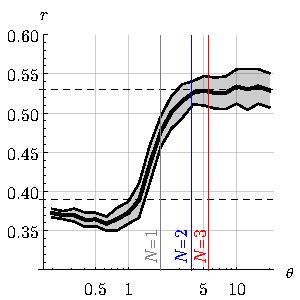
\includegraphics[align=c, width=0.225\textwidth]{imgs/ergodic_reg.pdf}
    \hspace{10 mm} 
    \addletter{50}{b}
    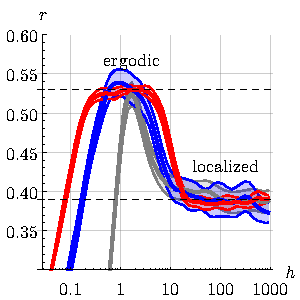
\includegraphics[align=c, width=0.225\textwidth]{imgs/transition.pdf}
    \hspace{5 mm} 
    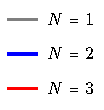
\includegraphics[align=c, width=0.075\textwidth]{imgs/transition_leg.pdf}
    \caption{
        a) The influence of matrix rarefaction $\theta$ on phase formation with $\xi = 0.01$. 
        b) Phase transition with 1D hard-bosons with $L=20$.
        }
    \label{fig:rtheta}
\end{figure}


I paid such attention to $\theta$ and fragmentation, since this in some sense helps to understand why for a small number of particles in the system the ergodic phase (judging by $r$) practically does not occur (fig. \ref{fig:rtheta}). Indeed, with a smaller number of particles ($N=1,2,3$) and the same lattice size $L=14$, the Hamiltonian is more rarefied (fig. \ref{fig:rtheta}a), Hilbert Space Fragmentation occurs (that is the Hamiltonian can be represented in block diagonal form) and, accordingly, thermalization does not occur.


The main conclusion of this section: the $r$-parameter is quite universal in nature and can be used as a marker of the ergodic phase and localized phase. The EP-LP phase transition can be modeled by random matrices (GOE, random diagonal, random graph adjacency matrix).





\begin{figure}[h]
    \centering
    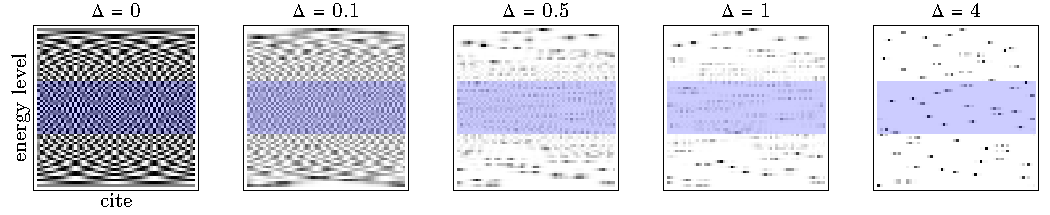
\includegraphics{imgs/evecs.pdf}
    \caption{
    The eigenstates $\ket{\psi_j}$ of the single-particle 1D Hamiltonian \eqref{9:model} onto gratings of length $L=60$, the color indicates the value $|\psi_j|^2$. It can be seen that localization occurs immediately for the ground state, but in the area highlighted in blue, localization occurs later.
    }
    \label{fig:loc1}
\end{figure}
